\subsection{Architektura}

W~tym rozdziale krótko przedstawiono architekturę projektowanego systemu. W~dalszej części niniejszej dokumentacji będzie to punkt odniesienia do sposobu działania aplikacji.

\begin{figure} [!ht]
    \centering
    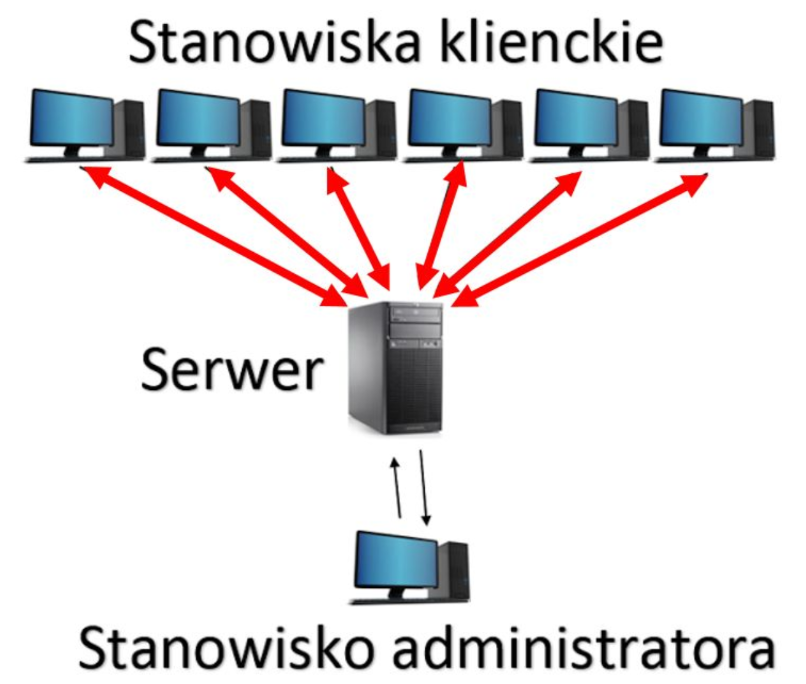
\includegraphics[height=8cm,width=10cm]{architektura}
    \caption{Projekt architektury systemu}
    \label{fig:architektura}
\end{figure}

Rysunek \ref{fig:architektura}. przedstawia architekturę projektowanego systemu. Stanowiska klienckie to komputery użytkowników np. w~sali komputerowej, na których uruchamiane są aplikacje klienckie. Stanowisko administratora, jest to komputer, który potrzebuje dostępu do przeglądarki internetowej, aby skorzystać z~aplikacji. Serwer natomiast udostępnia serwis internetowy, do którego łączą się administratorzy/nauczyciele i~stanowiska kliencie. Tutaj znajduje się także baza danych systemu.